%=============================================================================
% LATEX STUFF
% ============================================================================
\PassOptionsToPackage{table}{xcolor} % Enables colored tables cleanly
\documentclass{beamer}

\usepackage[orientation=portrait,size=a0,scale=1.4]{beamerposter}
\geometry{paperwidth=36in,paperheight=48in}

%=============================================================================
% OTHER PACKAGES
% ============================================================================
\usepackage[utf8]{inputenc}
\usepackage{amsmath,amssymb}
\usepackage{booktabs} % Elegant tables
\usepackage{helvet}
\renewcommand{\familydefault}{\sfdefault}
\usepackage{relsize}

%=============================================================================
% POSTER METADATA
% ============================================================================
\def\postertitle {Beyond Static Benchmarks: A Post-Leaderboard Evaluation Paradigm for Generative Music and Creative AI}
\def\posterauthor {Alexander Lerch}
\def\posteraffiliation {Music Informatics Group, Georgia Institute of Technology}
\def\posteraffiliationlink {\href{http://www.musicinformatics.org}{www.musicinformatics.org}}
\def\postercontactlink {\href{mailto:alexander.lerch@gatech.edu}{alexander.lerch@gatech.edu}}

%=============================================================================
% LAYOUT DEFINITIONS IN SEPARATE FILE
% ============================================================================
\input{layout}


% =============================================================================
% MAIN POSTER CONTENT
% =============================================================================
\begin{document}
\begin{frame}[t]
    \vspace{-7mm}
  
  \begin{columns}[t]
    % -------------------------------------------------------------------------
    % LEFT MARGIN
    % -------------------------------------------------------------------------
    \begin{column}{0.025\paperwidth}\end{column}

    % -------------------------------------------------------------------------
    % LEFT COLUMN
    % -------------------------------------------------------------------------
    \begin{column}{0.46\paperwidth}
      % \begin{block}{Music AI Evaluation: Current State}
      % \end{block}

      \begin{block}{Evaluation Crisis in Generative Music}
          The current state of evaluation in generative music is methodologically fragmented, relies on ambiguous validation objectives, and builds on systematically misaligned metrics \cite{lerch_survey_2025}. This has led to a crisis in the field, where the following failures are observed:
        
        \begin{itemize}
          \bigskip
          \item \textbf{Validity failure:}
              \begin{itemize}
                \item Utilized metrics are \textit{unreliable proxies} and fail to measure musical qualities.
              \end{itemize}
          \bigskip
          \item \textbf{Leaderboard failure:} 
              \begin{itemize}
                \item Single-score optimization leads to \textit{overfitting} and is \textit{insufficient for assessing a multi-dimensional cultural artifact}.
              \end{itemize}
          \bigskip
          \item \textbf{Comparability failure:} 
              \begin{itemize}
                \item \textit{Different metrics, feature representations, and reference data} prevent meaningful comparisons across models.
              \end{itemize}
          \bigskip
          \item \textbf{Reproducibility failure:}
             \begin{itemize}
                \item \textit{Closed-source representations and evaluation scripts} and proprietary data hinder reproducibility.
              \end{itemize}
          \bigskip
          \item \textbf{Governance failure:} 
             \begin{itemize}
                \item \textit{Ad-hoc, fragmented evaluation protocols} indicate lack of standardization.
              \end{itemize}
        \end{itemize}

      \end{block}

      \begin{block}{Goals of the Proposed Framework}
        \begin{itemize}
          \bigskip
          \item \textbf{Community-driven ecosystem governance:}
              \begin{itemize}
                \item coordinated by the community for the community. 
                \item metrics and evaluation protocols have to \textit{evolve with the field}.
              \end{itemize}
          \bigskip
          \item \textbf{Multi-dimensional evaluation:} 
              \begin{itemize}
                \item acknowledging the \textit{multi-dimensional nature of music}.
              \end{itemize}
          \bigskip
          \item \textbf{Interpretability:} 
              \begin{itemize}
                \item utilizing \textit{interpretable metrics} and features where possible.
              \end{itemize}
          \bigskip
          \item \textbf{Domain adaptability:}
             \begin{itemize}
                \item acknowledging \textit{variety of use cases} through curated reference benchmark profiles (RBPs).
              \end{itemize}
          \bigskip
          \item \textbf{Modularity \& extensibility:} 
             \begin{itemize}
                \item modular software architecture allows for easy \textit{integration of new features and evaluation methods}.
              \end{itemize}
          \bigskip
          \item \textbf{Reproducibility \& transparency:} 
             \begin{itemize}
                \item versioned \textit{open source} software with comprehensive documentation and \textit{auditable logging}.
              \end{itemize}
        \end{itemize}

      \end{block}

      \begin{block}{Governance Structure}
          \begin{figure}[!h]
            \centering
            \resizebox{.9\linewidth}{!}{\setlength{\unitlength}{1mm}
\tiny\relsize{-4}
\begin{picture}(91, 46)
  \setlength\fboxsep{0pt}
    
    

    
    % 1. Top
    \put(0, 26){\colorbox{white!20}{\framebox(91, 20){\shortstack{\textbf{Steering Committee}\\
      {\tiny\relsize{-6} overseeing framework development and maintenance,}\\ 
      {\tiny\relsize{-6} monitoring evaluation landscape,}\\ 
      {\tiny\relsize{-6} conducting ethics and IP reviews}}}}}
    
    % 2. TC
		% \put(0, 12){\framebox(24, 32){Data}}
  	\put(0, 0){\colorbox{white!20}{\framebox(24, 20){\shortstack{\textbf{Technical}\\ \textbf{Working Group}\\
      {\tiny\relsize{-6} maintains software,}\\ 
      {\tiny\relsize{-6} reproducibility reqs.}}}}}
     
    % 3. DPG
    \put(32, 0){\colorbox{white!20}{\framebox(24, 20){\shortstack{Domain\\Profile Groups}}}}
    \put(33, 1){\colorbox{white!20}{\framebox(24, 20){\shortstack{Domain\\Profile Groups}}}}
    \put(34, 2){\colorbox{white!20}{\framebox(24, 20){\shortstack{Domain\\Profile Groups}}}}
    \put(35, 3){\colorbox{white!20}{\framebox(24, 20){\shortstack{\textbf{Domain}\\\textbf{Profile Groups}\\
      {\tiny\relsize{-6} propose \& develop}\\ 
      {\tiny\relsize{-6} RBPs}}}}}
    
    % 4. Community Review
    \put(67, 0){\colorbox{white!20}{\framebox(24, 20){\shortstack{\textbf{Community}\\\textbf{Review Process}\\
      {\tiny\relsize{-6} proposal,}\\ 
      {\tiny\relsize{-6} public comment,}\\ 
      {\tiny\relsize{-6} deprecation policy.}}}}}
    
    % --- ARROWS & CONNECTORS ---
    
    % Evaluation Profiles Downward Links
    \put(12, 20){\vector(0,1){6}}    % Ref -> Log
    \put(44, 23){\vector(0,1){3}}   % Feat -> Log
     
    % Main Pipeline Flow
    {\linethickness{1.5pt}
    
     \put(24,14){\vector(1,0){8}}     % From TC to DPG
     \put(32, 6){\vector(-1,0){8}}
    
     \put(59, 14){\vector(1,0){8}}     % From feat Data
     \put(67, 6){\vector(-1,0){8}}     % From feat Data
    
    }
\end{picture}
}
            \caption{Proposed governance structure}
          \end{figure}
      \end{block}
    \end{column}
    
    % -------------------------------------------------------------------------
    % MIDDLE SPACER
    % -------------------------------------------------------------------------
    \begin{column}{0.025\paperwidth}\end{column}
    
    % -------------------------------------------------------------------------
    % RIGHT COLUMN
    % -------------------------------------------------------------------------
    \begin{column}{0.46\paperwidth}
      \begin{block}{Architecture}
          \begin{figure}[!h]
            \centering
            \resizebox{.9\linewidth}{!}{\setlength{\unitlength}{1mm}
\tiny\relsize{-4}
\begin{picture}(142, 56)
  \setlength\fboxsep{0pt}
    % --- COORDINATE DEFINITIONS ---
    % Horizontal centers: C1=20, C2=65, C3=110, C4=155
    % Vertical centers: Top=100, Gen=75, Mid=50, Ref=25, Log=5
    
    % --- BOX DIMENSIONS ---
    % Standard Box: 30x16
    
    % 1. EVALUATION PROFILES (Top)
    \put(0, 48){\colorbox{white!20}{\framebox(142, 8){(Governed) Reference Benchmark Profiles}}}
    \put(33, 50){
\includegraphics[scale=.2]{graph/rbp}}
    
    % 2. INPUT DATA (Left Column)
		% \put(0, 12){\framebox(24, 32){Data}}
  	\put(0, 12){\colorbox{gray!10}{\framebox(24, 32){Data}}}
    \put(2, 34){\colorbox{white!20}{\framebox(20, 8){Reference}}}
    \put(2, 14){\colorbox{white!20}{\framebox(20, 8){Generated}}}
    \put(18, 29){
\includegraphics[scale=.25]{graph/data}}
    \put(18, 23){
\includegraphics[scale=.25]{graph/data}}
    
    % 3. FEATURE EXTRACTION
    \put(32, 12){\colorbox{white!20}{\framebox(24, 32){\shortstack{Feature\\Extraction}}}}
    \put(42, 32){
\includegraphics[scale=.2]{graph/featureextract}}
    
    % 4. DISTRIBUTION SYMBOL (Replacing the box)
    % Drawing a Bell Curve
    \put(65, 36){\qbezier(0,0)(5,10)(10,0)}
    \put(66, 37){\qbezier(0,0)(5,10)(10,0)}
    \put(67, 38){\qbezier(0,0)(5,10)(10,0)}
    
    \put(65, 16){\qbezier(0,0)(5,10)(10,0)}
    \put(66, 17){\qbezier(0,0)(5,10)(10,0)}
    \put(67, 18){\qbezier(0,0)(5,10)(10,0)}
		%\put(65, 16){\qbezier(0,0)(7.5,15)(15,0)}
    %\put(95, 50){\line(1,0){15}}
    \put(64, 30){\makebox(13,0)[c]{ Distributions}}

    % 5. DISTANCE METRIC
    \put(86, 12){\colorbox{white!20}{\framebox(24, 32){\shortstack{Distance\\Metric}}}}
    \put(96, 32){
\includegraphics[scale=.2]{graph/distance}}
    
    % 6. VISUALIZATION (Right)
    \put(118, 12){\colorbox{white!20}{\framebox(24, 32){\shortstack{Multidim. Eval.,\\Visualization}}}}
    \put(128, 32){
\includegraphics[scale=.2]{graph/visual}}
    
    % 7. LOGGING (Bottom)
    \put(0, 0){\colorbox{white!20}{\framebox(110, 8){Logging (JSON, PDF, \ldots)}}}
    \put(33, 3){
\includegraphics[scale=.2]{graph/log}}

    % --- ARROWS & CONNECTORS ---
    
    % Evaluation Profiles Downward Links
    \put(12, 48){\vector(0,-1){4}}    % Ref -> Log
    \put(44, 48){\vector(0,-1){4}}   % Feat -> Log
    \put(98, 48){\vector(0,-1){4}}  % Metric -> Log
    \put(130, 48){\vector(0,-1){4}}  % Metric -> Log
      
    % Main Pipeline Flow
    {\linethickness{1.5pt}
    \put(24, 38){\vector(1,0){8}}     % From ref Data
    %\put(42.5, 75){\vector(1,-2){7.5}} % Slant to Feature Extraction
    
    \put(24, 18){\vector(1,0){8}}     % From gen Data
    %\put(42.5, 25){\vector(1,2){7.5}}  % Slant to Feature Extraction

    \put(56, 38){\vector(1,0){8}}     % From feat Data
    \put(56, 18){\vector(1,0){8}}     % From feat Data

    \put(78, 38){\vector(1,0){8}}     % From dist Data
    \put(78, 18){\vector(1,0){8}}     % From dist Data

    %\put(80, 50){\vector(1,0){15}}    % Feat -> Dist
    %\put(110, 50){\vector(1,0){20}}   % Dist -> Metric
    \put(110, 30){\vector(1,0){8}}  % Metric -> Viz
    }
    % Logging Downward Links
    \put(12, 12){\vector(0,-1){4}}    % Ref -> Log
    \put(44, 12){\vector(0,-1){4}}   % Feat -> Log
    \put(98, 12){\vector(0,-1){4}}  % Metric -> Log

\end{picture}
}
            \caption{Proposed framework architecture for the evaluation of generative music.}
          \end{figure}
        
        \vskip2ex
        \begin{itemize}
          \item \textbf{Reference Benchmark Profiles (RBPs):}
              \begin{itemize}
                \item use-case specific combination of \textit{reference data}, \textit{feature representations}, and \textit{distance metrics}, and \textit{reporting format}.
              \end{itemize}
          \bigskip
          \item \textbf{Standardized Reference Data:} 
              \begin{itemize}
                \item publicly available, documented datasets as controllable open references.
              \end{itemize}
          \bigskip
          \item \textbf{Standardized Feature Representations:} 
              \begin{itemize}
                \item musical qualities
                \item audio fidelity
                \item controllability
                \item originality
              \end{itemize}
          \bigskip
          \item \textbf{Standardized Distance Metrics:} 
              \begin{itemize}
                \item distributional distance metrics (Wasserstein, KL, MMD, etc.)
                \item traditional evaluation metrics (accuracy, precision, recall, F1, etc.) for classification tasks
                \item task-specific metrics as needed
              \end{itemize}
          \bigskip
          \item \textbf{Multi-dimensional Results \& Visualization:}
              \bigskip
              
              \begin{figure}[!h]
                \centering
                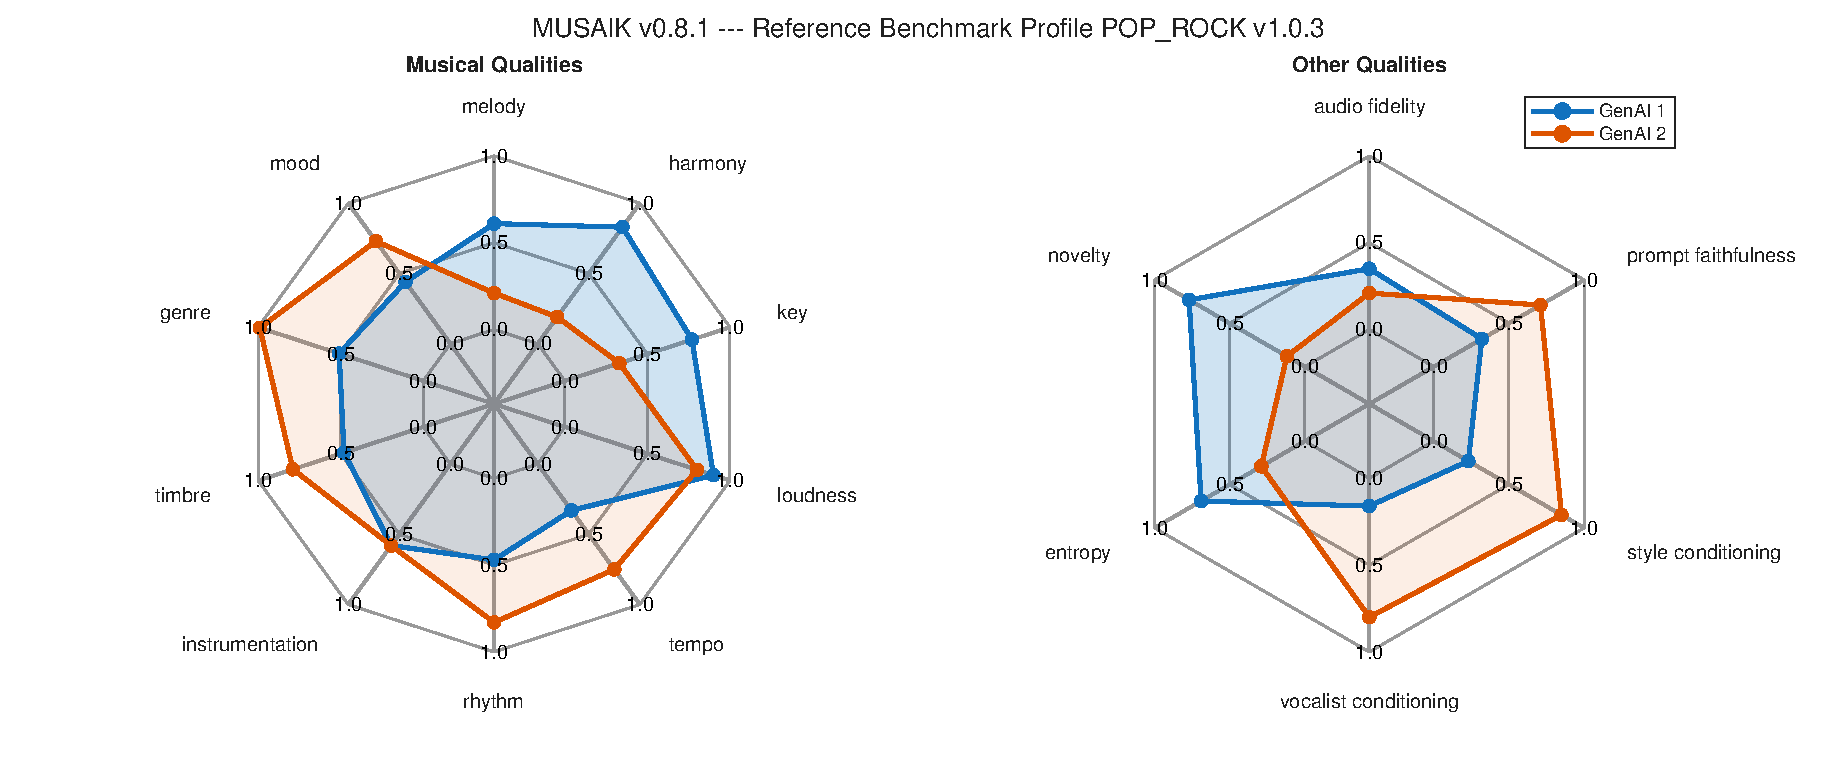
\includegraphics[width=.5\linewidth]{graph/Mockup.pdf}
                \caption{Mockup of aggregated result presentation.}
              \end{figure}
'           \bigskip
            \item \textbf{Logging:}
              \begin{itemize}
                \item auditable logs (machine \& human readable formats) with RBP, version info, test data, etc.
              \end{itemize}
        \end{itemize}
      \end{block}

      \begin{block}{Limitations}
        \begin{itemize}
            \item Missing \textbf{subjective evaluation protocols}
            \bigskip
            \item \textbf{Black-box evaluation}:
              \begin{itemize}
                  \item no evaluation of the underlying model architecture/capabilities
                  \item no distinction between human contributions and fully machine-generated output
              \end{itemize}
           \bigskip
            \item \textbf{Focus on output qualities}:
              \begin{itemize}
                \item no usability or user experience evaluation
                \item no evaluation other characteristics, such as explainability, bias, resource usage, ethical use of data, etc.
              \end{itemize}
        \end{itemize}
      \end{block}

      \begin{block}{Cross-Domain Applicability}
          \begin{itemize}
            \item easily transferable to other domains of generative AI, such as \textbf{Visual Art}, \textbf{Text Generation}, and \textbf{Game Content Generation}
            \item modular architecture $\Rightarrow$ \textbf{exchange feature representations}.
          \end{itemize}
      \end{block}

      \begin{block}{References}
        \footnotesize
        \bibliographystyle{plain}
        \bibliography{2026-AI-Benchmark}

        % \vskip1ex
        % \scriptsize \color{GTGrayMatter}
        % Acknowledgment: This production environment was developed inside the ECE Senior Design and Research ecosystems at Georgia Institute of Technology.
      \end{block}
    \end{column}
    
    % -------------------------------------------------------------------------
    % RIGHT MARGIN
    % -------------------------------------------------------------------------
    \begin{column}{0.025\paperwidth}\end{column} 
  \end{columns}
\end{frame}
\end{document}